\documentclass[runningheads]{llncs}

\usepackage{graphicx}
\usepackage{placeins}
\usepackage{hyperref,xcolor}
\renewcommand\UrlFont{\color{blue}\rmfamily}
\usepackage{listings}
\definecolor{very-light-gray}{gray}{0.95}

\begin{document}

\title{Solving Combinatorial Puzzles with Parallel Evolutionary Algorithms \thanks{This work was supported by a private funding of Velbazhd Software LLC.}}
\titlerunning{Solving Puzzles with PEA}

\author{Todor Balabanov\orcidID{0000-0003-3139-069X} \and
Stoyan Ivanov \and
Rumen Ketipov}
\authorrunning{T. Balabanov et al.}

\institute{Institute of Information and Communication Technologies \\
Bulgarian Academy of Sciences \\
acad. Georgi Bonchev Str., Block 2, 1113 Sofia, Bulgaria \\
\email{todorb@iinf.bas.bg} \\
\url{http://iict.bas.bg/}}

\maketitle

\begin{abstract}
Rubik's cube is the most popular combinatorial puzzle. It is well known that solutions of the combinatorial problems are generally hard to find. If 90 degree clockwise rotations of the cube's sides are taken as operations it will give a minimal cube's grammar. By building formal grammar sentences with the usage of the six operations ([L]eft, [R]ight, [T]op, [D]own, [F]ront, [B]ack) all cube's permutations can be achieved. In an evolutionary algorithms (like genetic algorithms for example) set of formal grammar sentences can be represented as population individuals. Single cut point crossover can be efficiently applied when population individuals are strings. Changing randomly selected operation with another randomly selected operation can be used as efficient mutation operator. The most important part of such global optimization is the fitness function. For better individuals fitness value evaluation a combination between Euclidean and Hausdorff distances is proposed in this research. The experiments in this research are done as parallel program written in C++ and Open MPI.

\keywords{Distributed evolutionary algorithms \and Combinatorial puzzles \and Integer optimization.}
\end{abstract}

\section{Introduction}

A parallel implementation of a genetic algorithm-based solver of the Rubik's cube was implemented by Balabanov in \cite{balabanov01} and it was presented in \cite{balabanov02}. Rubik's cube was invented and introduced by Erno Rubik in the 70s of the 20th century. After its creation the cube became the most popular combinatorial puzzle all over the world. In its original version it has 3x3x3 cubical segments. There are stickers in six different colors on each subcube square of the exposed sides. Each of the six planes (3x3x1) can be rotated in 90, 180, 270 or 360 degrees, relative to the other part of the puzzle. In the original initial state all sides of the cube are in single color. Scumbling of the puzzle is done by many random rotations of the (3x3x1) sides. The optimization task aims to restore the cube in its original state. Such combinatorial optimization problem is quite difficult because there are billions of combinations. The real number of combinations is $4.3252*10^{19}$ \cite{korf01} and all of them can be reached from any starting combination. The puzzle is successfully resolved when a sequence of moves is applied such that all subcubes are matched to each other by their color on each side of the cube. According to an estimation in \cite{korf01} resolutions sequences variate from 50 to 100 moves when the cube is well scrambled. 

When there is an optimization problem with a sequence of commands it is a perfect candidate for evolutionary algorithms as optimizers. This research addresses the application of parallel genetic algorithms for Rubik's cube optimal or suboptimal solutions findings. The source code of the experiments is written in C++ with OpenMPI for parallel calculations and it can be found in a public source code repository \cite{balabanov01}. Modification of the evaluation function presented in \cite{balabanov02} is upgraded by addition of Hausdorff distance component.

The rest of this paper is organized as follows: Section 2 briefly describes theoretical details. Hence, section 3 presents the proposed modifications into a practical software example and section 4 is devoted to some experiments and results. Finally, Section 5 concludes and presents some ideas for further research.

\section{Parallel Genetic Algorithms}

Genetic algorithms are global optimization strategy inspired from the evolution process in the Biology theories. Place of the genetic algorithms and the genetic programming in the family of the metaheuristics is well presented in Fig.\ref{fig02}.

\begin{figure}
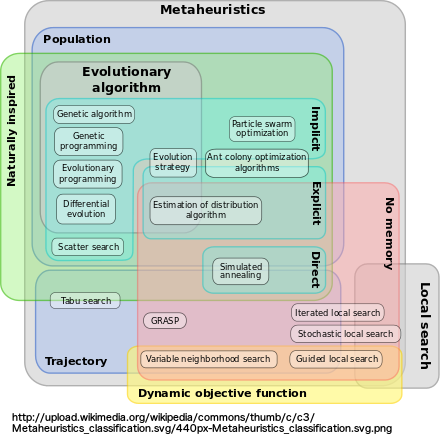
\includegraphics[width=1.0\textwidth,height=0.65\textwidth]{fig02.png}
\centering
\caption{Euler diagram of the different classifications of metaheuristics.} \label{fig02}
\end{figure}
%\FloatBarrier

Solutions of a particular problem are represented as vectors of values into the solution space. All selected solution vectors are the population of the algorithm. The most common way of initial population establishment is by generation of random vectors. Each new generation appears in the population after recombination of selected individuals. In genetic algorithms recombination is done by two consequent operators - crossover and mutation. Which individuals to participate in the recombination process is decided by application of selection operator. It is very common during selection process elitism rule to be applied. Elitism means that some percent of the best found solutions survive to the real end of the optimization process. Because genetic algorithms based optimization is an iterative optimization a stopping criteria is needed. The most used stopping criteria is initially given number of genetic algorithm generations. 

Genetic algorithms are the base of the genetic programming which is used in this research. Each element of the solution vector actually is an operation applied over the state of the Rubik's cube. Ordered set of such instructions is actually an algorithmic program. Because there is no direct intermediate relation between the individuals in a particular population genetic algorithms are highly appropriate for implementation in parallel computing or distributed computing. Population of the genetic algorithm can be easily divided in many sub-population and it can be distributed on many processors/cores or even heterogeneous computers in a cluster. Separation of the global population is the preferred approach, but in cases where only the fitness value calculation is time consuming, population is kept in the central processor/computer and only fitness value calculation is sent to the other contributing processors/computers. 

When sub-populations distribution calculation scheme is selected some strategy for individual migration should be applied \cite{balabanov02}. Migration between different islands is needed in order best found solutions to be available in some or in all sub-populations. When the implementation of the calculation is organized as donated distributed computing project in the inclusion of a new remote contributing computer fresh subset of the global population can be supplied. With such strategy solutions space is much better investigated. 

\section{Modified Rubik's Cube Solver}

The core of the optimization code is Rubik's cube representation into the computer memory. For the needs in this research the cube is presented as six (one for each side) two-dimensional (3x3) arrays. Values in these arrays are integer numbers which correspond to cube's colors. There are better ways for digital representation \cite{korf01}, but it is much more practical in this way from algorithmic aspect. 

Data structures are the first side of the modeling proccess. On the second side are the algorithmic operations done over the data structures. The cube has six sides that is why the minimum number of operations over the cube is six. Six capital letters are used for 90 degrees clockwise rotations, as proposed in \cite{randall01,balabanov02}: \\ 
\\
T (Top) –90 degrees clockwise rotation of the top side; \\ 
L (Left) –90 degrees clockwise rotation of the left side; \\ 
B (Back) –90 degrees clockwise rotation of the back side; \\ 
R (Right) –90 degrees clockwise rotation of the right side; \\ 
F (Front) –90 degrees clockwise rotation of the front side; \\ 
D (Down) –90 degrees clockwise rotation of the down side. \\ 

This set of six operations is the minimal fully functional grammar for the Rubik's cube. Extended grammars are also possible, for example if counter-clockwise operators are included (+T, +L, +B, +R, +F, +D, –T, –L, –B, –R, –F, –D). Next level of extension is addition as number of turns (+1T, +2T, +3T, +1L, +2L, +3L, +1B, +2B, +3B, +1R, +2R, +3R, +1F, +2F, +3F, +1D,+2D, +3D, –1T, –2T, –3T, –1L, –2L, –3L, –1B, –2B, –3B, –1R, –2R, –3R, –1F, –2F, –3F, –1D, –2D, –3D) \cite{balabanov02}.

With the presented ideas for a formal Rubik's cube grammar the neutral choice is genetic algorithm individuals to be represented as formal grammar sentences with variable length. Each of the letters can appear at any position many times repeated in the chromosome. As it was appointed in \cite{korf01} the average expected length of the chromosomes can be between 50 and 100.

\begin{figure}
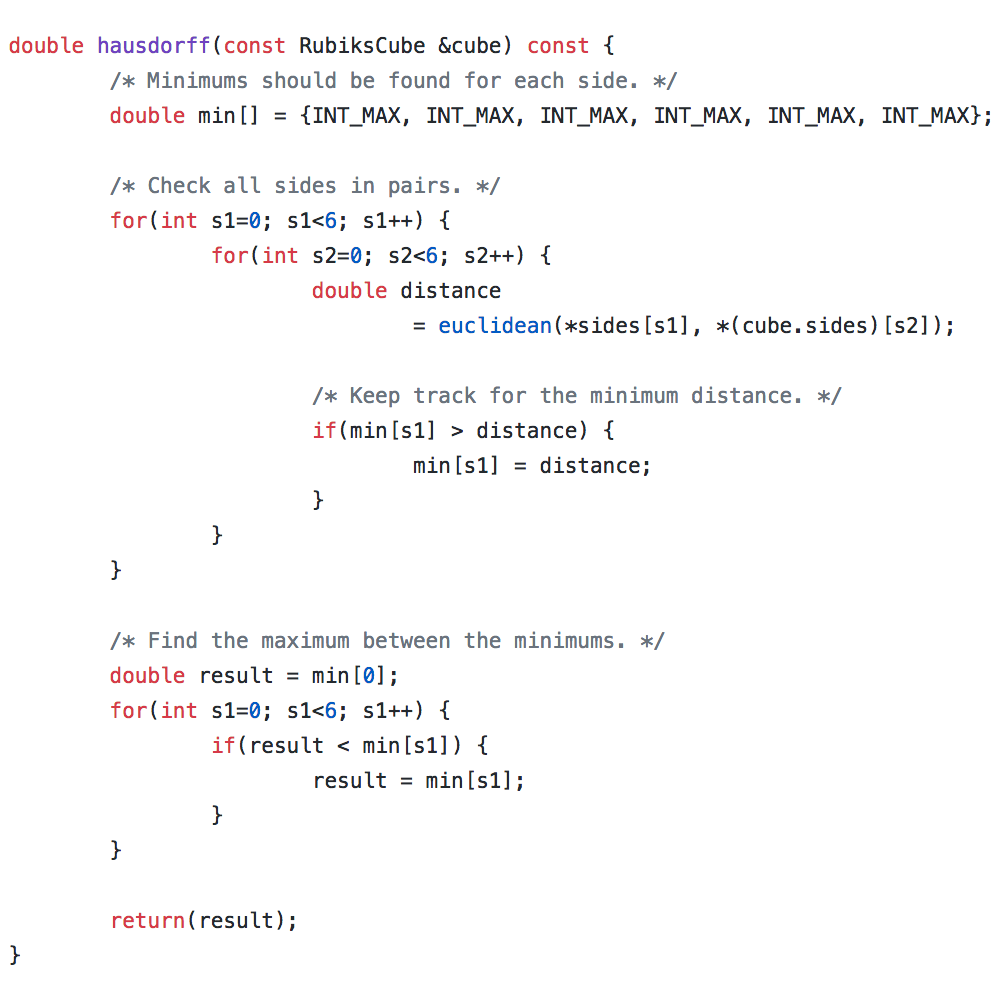
\includegraphics[width=0.75\textwidth]{fig01.png}
\centering
\caption{Fitness value evaluation by combination between Euclidean and Hausdorff distance.} \label{fig01}
\end{figure}
\FloatBarrier

Single cut point is selected as crossover population, but other options \cite{poli01} are also applicable. As mutation operator random change of a single instruction is selected. Selection is done by randomly selected parents, but elitism rule is applied. For the evaluation of the newly created individuals instructions encoded in the individual are applied over the scrambled cube. After that the state of the cube is compared with the target state (cube in the solved state). The listing in Fig.\ref{fig01} shows the proposed in this paper modification of fitness evaluation function. For each pairs of cube's sides Euclidean distance is calculated. After that according to Hausdorff distance rules the maximum of the minimums is found. Evaluated fitness value is positive because the Euclidean distance is calculated with positive integers (cube's colors are mapped to integers) and the Hausdorff distance is a calculation of a maximum of the minimums. The puzzle is as better solved as the fitness value is smaller. 

\section{Experiments and Results}

All experiments were done on a single processor desktop machine - Intel Core i5, 2.3 GHz, 2 Cores, 8GB RAM and Mac OS X 10.13.6, Apple LLVM version 9.1.0. For the parallel implementation Open MPI is used.

\begin{figure}
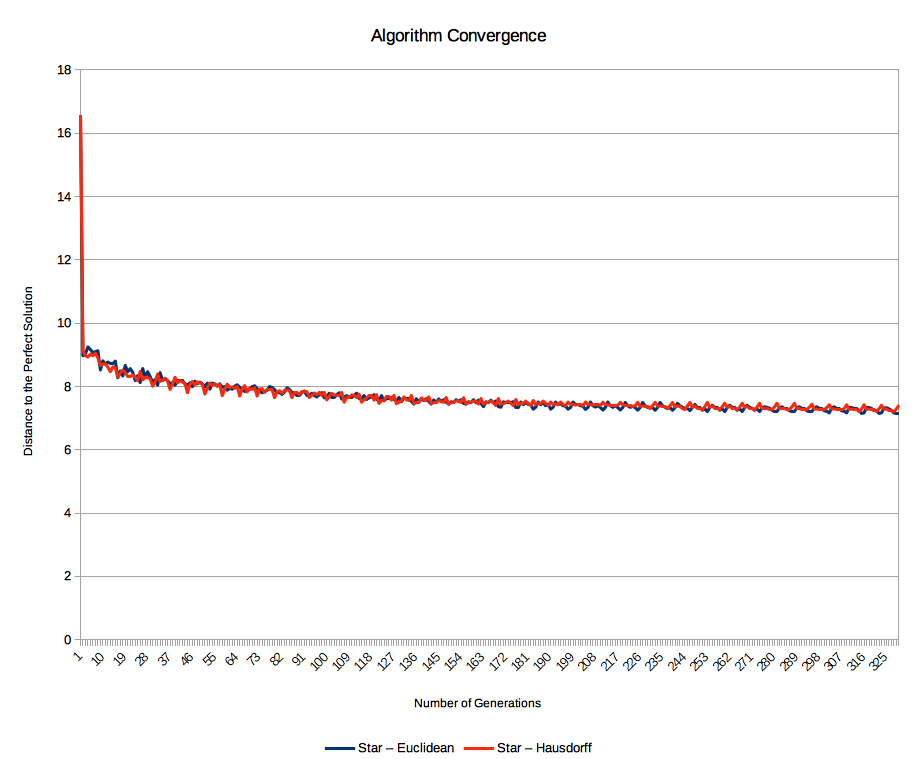
\includegraphics[width=0.75\textwidth]{fig03.png}
\centering
\caption{Algorihtm convergence with star topology.} \label{fig03}
\end{figure}
\FloatBarrier

Experiments are done in two groups with 30 independent runs for each. The source code originally is divided for test with star topology and incident nodes participation as migration strategies. That is why there are two groups of experiments. Each experiment compares pure Euclidean distance implementation and the proposed Hausdorff distance modification. Parameters of the genetic algorithm are listed in Tab. \ref{tab01}.

\begin{table}
\caption{Genetic algorithm parameters.}
\label{tab01}
\begin{tabular}{p{6.9cm}p{4.4cm}}
\hline\noalign{\smallskip}
\textbf{Parameter} & \textbf{Value} \\
\hline\noalign{\smallskip}
generation gap & 0.93 \\
crossover rate & 0.98 \\
mutation rate & 0.01 \\
maximum generations & 10000 \\
number of individuals & 37 \\
number of variables & floating \\
inserted rate & 100 \% \\
\noalign{\smallskip}\hline\noalign{\smallskip}
\end{tabular}
\end{table}
\FloatBarrier

\begin{figure}
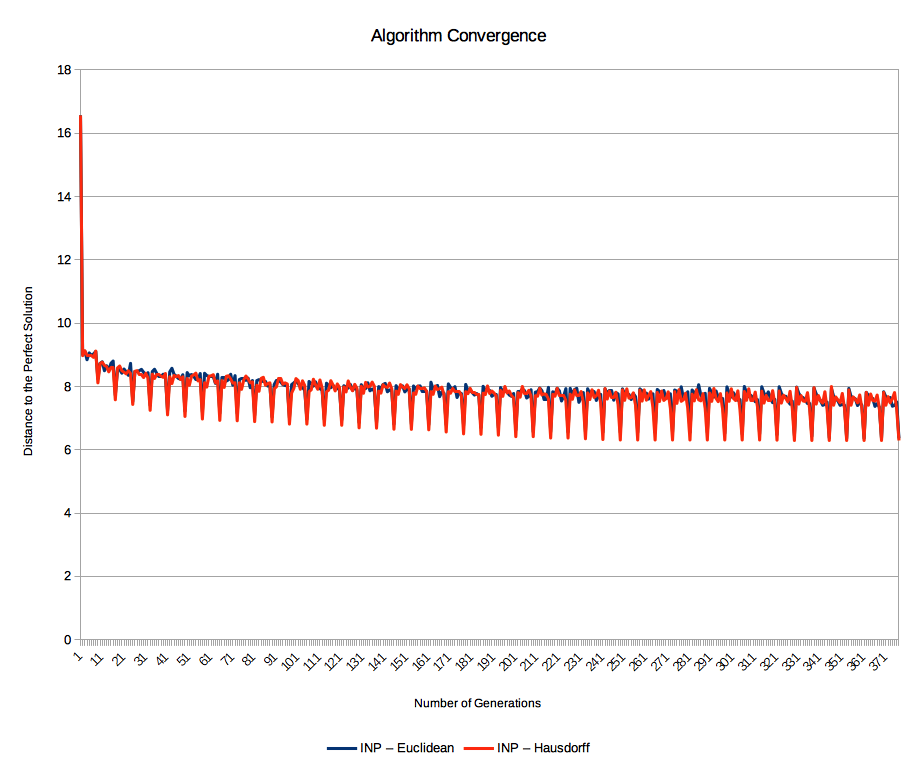
\includegraphics[width=0.75\textwidth]{fig04.png}
\centering
\caption{Algorihtm convergence with incident nodes participation.} \label{fig04}
\end{figure}
\FloatBarrier

Fig.\ref{fig03} shows that when star topology is used the advantage of Hausdorff modification is not so great, but as it is shown in Fig.\ref{fig04} when an incident nodes participation is used the proposed modification leads to convergence seep-up. Calculation of a Euclidean distance between two cubes uses six calculations of the sides for the cube (Listing \ref{lst01}). In the case of Hausdorff distance there are six times more calls of a single Euclidean distance calculation (Listing \ref{lst02}).

\begin{lstlisting}[caption={Euclidean distance.},label={lst01},backgroundcolor=\color{very-light-gray},frame={single}]
double euclidean(const int side1[3][3], 
                 const int side2[3][3]) const {
  double distance = 0.0;

  for(int i=0; i<3; i++) {
    for(int j=0; j<3; j++) {
      distance += (side1[i][j]-side2[i][j]) * 
                  (side1[i][j]-side2[i][j]);
    }
  }

  return sqrt(distance);
}
\end{lstlisting}
\FloatBarrier

\begin{lstlisting}[caption={Hausdorff distance.},label={lst02},backgroundcolor=\color{very-light-gray},frame={single}]
double hausdorff(const RubiksCube &cube) const {
  double min[] = {INT_MAX, INT_MAX, INT_MAX, 
                  INT_MAX, INT_MAX, INT_MAX};

  for(int s1=0; s1<6; s1++) {
    for(int s2=0; s2<6; s2++) {
      double distance = 
      euclidean(*sides[s1], *(cube.sides)[s2]);

      if(min[s1] > distance) {
        min[s1] = distance;
      }
    }
  }

  double result = min[0];
  for(int s1=0; s1<6; s1++) {
    if(result < min[s1]) {
      result = min[s1];
    }
  }

  return(result);
}
\end{lstlisting}
\FloatBarrier

\section{Conclusions}

The experiments show that the addition of Hausdorff distance component improves the performance of the genetic algorithm. A calculation of the Hausdorff distance is a little bit slower than the calculation of the Euclidean distance, but better solution fitness estimation generally leads to genetic algorithm convergence improvement. Further investigations in the field of the soft computing can be done for the proposed fitness value evaluation as it was done in \cite{angelova01}.

As further research it will be interesting an evaluation of the fitness value to be additionally filtered with Kalman filter \cite{alexandrov01}, for example. Another interesting direction would be an involvement of the artificial neural networks such as \cite{tashev01,atanasova01} for preliminary solutions evaluation.

\begin{thebibliography}{8}
\bibitem{balabanov01}
MPI Parallel Implementation of Genetic Algorithm Based Rubik’s Cube Solver, \url{http://github.com/TodorBalabanov/RubiksCubeGeneticAlgorithmsSolver}. Last accessed 10 Feb 2019
\bibitem{balabanov02}
Balabanov, T., Zankinski, I., Barova, M.: Strategy for Individuals Distribution by Incident Nodes Participation in Star Topology of Distributed Evolutionary Algorithms. Cybernetics and Information Technologies \textbf{16}(1), 80--88 (2016)
\bibitem{korf01}
Korf, R.: Finding Optimal Solutions to Rubik’s Cube Using Pattern Databases. In: AAAI-98 Proceedings, pp. 700--705. AAAI Press, Menlo Park, CA, USA (1998)
\bibitem{randall01}
Randall, K.: Cilk - Efficient Multithreaded Computing. Doctor of Philosophy Thesis in Computer Science and Engineering, Massachusetts Institute of Technology, USA (1998) 
\bibitem{poli01}
Poli, R., Kozak J.: Genetic Programming. In: Burke, EK., Kendall, G. (eds.) Search Methodologies, pp. 143--185. Springer US (2014)
\bibitem{angelova01}
Angelova, V.: Investigations in the Area of Soft Computing Targeted State of the Art Report. Cybernetics and Information Technologies \textbf{9}(1), 18--24 (2009)
\bibitem{alexandrov01}
Alexandrov, A.: AD HOC Kalman filter based fusion algorithm for real-time Wireless Sensor Data Integration. In: FQAS-2015 Proceedings, pp. 151--160. Springer, Heidelberg (2015)
\bibitem{tashev01}
Tashev, T., Hristov, H.: Modeling of synthesis of information processes with generalized nets. Cybernetics and Information Technologies, \textbf{3}(2), 92--104 (2003) 
\bibitem{atanasova01}
Atanasova T., Barova M.: Exploratory analysis of Time Series for hypothesize feature values. In: UniTech17 Proceedings,  \textbf{16}(2), 399--403 (2017)
\end{thebibliography}
\end{document}
